\documentclass[10pt,aspectratio=169,serif]{beamer}

\usepackage[fontset=none, scheme=plain]{ctex}
\IfFontExistsTF{Songti SC}{%
	\setCJKmainfont{Songti SC}[AutoFakeSlant=0.2]%
	\setCJKsansfont{Songti SC}[AutoFakeSlant=0.2]%
}{%
	\setCJKmainfont{FandolSong-Regular}[Extension=.otf,BoldFont=FandolSong-Bold,AutoFakeSlant=0.2]%
	\setCJKsansfont{FandolSong-Regular}[Extension=.otf,BoldFont=FandolSong-Bold]%
}
\usepackage{amsmath,amssymb,graphicx,tikz,booktabs,multicol,calligra}
\usepackage{pgfplots}
\pgfplotsset{compat=1.18}
\usepackage{tcolorbox}
\tcbuselibrary{skins}
\usepackage{XyygU}
\usepackage{caption}
\captionsetup[figure]{name=图,labelsep=period}

\usetikzlibrary{arrows.meta,positioning,calc}

\setlength{\abovedisplayskip}{0pt plus 2pt minus 2pt}
\setlength{\belowdisplayskip}{0pt plus 2pt minus 2pt}

\title[习题5.4]{习题 5.4　三角函数的图象与性质}
\subtitle{复习巩固 \& 综合运用 \& 拓广探索}
\author{}
\institute{}
\date{2026-10-16}

\begin{document}

\begin{frame}
  \titlepage
\end{frame}

% ================= 复习巩固 =================
\begin{frame}[c]\Huge\centering 复习巩固\end{frame}

% ---------- 1 ----------
\begin{frame}[t]{复习巩固 1：画简图}
\textbf{1.} 画出下列函数的简图：
\begin{enumerate}[(1)]
  \item $y=1-\sin x$，$x\in[0,2\pi]$； \qquad
  \item $y=3\cos x+1$，$x\in[0,2\pi]$。
\end{enumerate}
\end{frame}

\begin{frame}[t]{复习巩固 1 解答}
\begin{columns}
\begin{column}{0.55\textwidth}
\small
五点列表（$x=0,\frac\pi2,\pi,\frac{3\pi}{2},2\pi$）：
\begin{tabular}{c|ccccc}
$y=1-\sin x$ & $1$ & $0$ & $1$ & $2$ & $1$\\
\hline
$y=3\cos x+1$ & $4$ & $1$ & $-2$ & $1$ & $4$\\
\end{tabular}
\vspace{0.5em}
\small
按五点描点、连线即得简图（分别由 $y=-\sin x$ 上移 $1$、$y=3\cos x$ 上移 $1$ 得到）。
\end{column}
\begin{column}{0.45\textwidth}
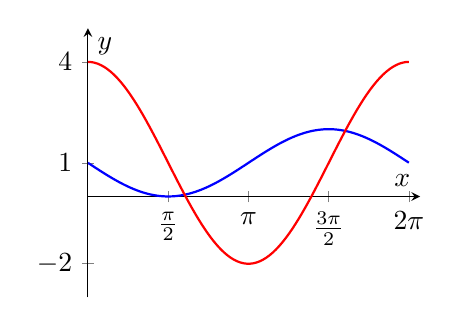
\begin{tikzpicture}
\begin{axis}[
    width=5.8cm, height=5cm,
    axis lines=middle, xlabel={$x$}, ylabel={$y$},
    xmin=0, xmax=6.5, ymin=-3, ymax=5,
    xtick={1.57,3.14,4.71,6.28},
    xticklabels={$\frac\pi2$,$\pi$,$\frac{3\pi}{2}$,$2\pi$},
    ytick={-2,1,4},
]
\addplot[thick,blue,domain=0:6.28,samples=100] {1-sin(deg(x))};
\addplot[thick,red,domain=0:6.28,samples=100] {3*cos(deg(x))+1};
\end{axis}
\end{tikzpicture}
\end{column}
\end{columns}
\end{frame}

% ---------- 2 ----------
\begin{frame}[t]{复习巩固 2：求周期}
\textbf{2.} 求下列函数的周期：
\begin{enumerate}[(1)]
  \item $y=\sin\dfrac{2x}{3}$，$x\in\mathbf R$； \qquad
  \item $y=\dfrac12\cos 4x$，$x\in\mathbf R$。
\end{enumerate}
\end{frame}

\begin{frame}[t]{复习巩固 2 解答}
\begin{tcolorbox}[colback=orange!10,colframe=orange,title=\textbf{解}]
$y=A\sin(\omega x+\varphi)$、$y=A\cos(\omega x+\varphi)$ 的最小正周期为 $T=\dfrac{2\pi}{|\omega|}$。
\vspace{0.3em}
(1) $\omega=\dfrac23$，$T=\dfrac{2\pi}{2/3}=\alert{3\pi}$；
\vspace{0.3em}
(2) $\omega=4$，$T=\dfrac{2\pi}{4}=\alert{\dfrac{\pi}{2}}$。
\end{tcolorbox}
\end{frame}

% ---------- 3 ----------
\begin{frame}[t]{复习巩固 3：奇偶性}
\textbf{3.} 下列函数中，哪些是奇函数？哪些是偶函数？哪些既不是奇函数，也不是偶函数？
\begin{enumerate}[(1)]
  \item $y=|\sin x|$； \qquad
  \item $y=1-\cos 2x$； \qquad
  \item $y=-3\sin 2x$； \qquad
  \item $y=1+2\tan x$。
\end{enumerate}
\end{frame}

\begin{frame}[t]{复习巩固 3 解答}
\begin{tcolorbox}[colback=orange!10,colframe=orange,title=\textbf{解}]
(1) $|\sin(-x)|=|-\sin x|=|\sin x|$，\alert{偶函数}；
\vspace{0.3em}
(2) $1-\cos(-2x)=1-\cos2x$，\alert{偶函数}；
\vspace{0.3em}
(3) $-3\sin(-2x)=3\sin2x=-(-3\sin2x)$，\alert{奇函数}；
\vspace{0.3em}
(4) $1+2\tan(-x)=1-2\tan x$，与 $1+2\tan x$ 既不相等也不相反，\alert{既不是奇函数也不是偶函数}。
\end{tcolorbox}
\end{frame}

% ---------- 4 ----------
\begin{frame}[t]{复习巩固 4：最值与对应自变量}
\textbf{4.} 求使下列函数取得最大值、最小值的自变量 $x$ 的集合，并求出最大值、最小值：
\begin{enumerate}[(1)]
  \item $y=1-\dfrac12\cos\dfrac{\pi x}{3}$； \qquad
  \item $y=3\sin\!\left(2x+\dfrac{\pi}{4}\right)$；
  \item $y=-\dfrac32\cos\!\left(\dfrac12x-\dfrac{\pi}{6}\right)$； \qquad
  \item $y=\dfrac12\sin\!\left(\dfrac12x+\dfrac{\pi}{3}\right)$。
\end{enumerate}
\end{frame}

\begin{frame}[t]{复习巩固 4 解答}
\begin{tcolorbox}[colback=orange!10,colframe=orange,title=\textbf{解}]
(1) $\cos\dfrac{\pi x}{3}=1$（$x=6k$）时 $y_{\min}=\dfrac12$；$\cos\dfrac{\pi x}{3}=-1$（$x=3+6k$）时 $y_{\max}=\dfrac32$。
\vspace{0.2em}
(2) $2x+\dfrac\pi4=\dfrac\pi2+2k\pi$（$x=\dfrac\pi8+k\pi$）时 $y_{\max}=3$；$2x+\dfrac\pi4=-\dfrac\pi2+2k\pi$（$x=-\dfrac{3\pi}{8}+k\pi$）时 $y_{\min}=-3$。
\vspace{0.2em}
(3) $\dfrac12x-\dfrac\pi6=\pi+2k\pi$（$x=\dfrac{7\pi}{3}+4k\pi$）时 $y_{\max}=\dfrac32$；$\dfrac12x-\dfrac\pi6=2k\pi$（$x=\dfrac\pi3+4k\pi$）时 $y_{\min}=-\dfrac32$。
\vspace{0.2em}
(4) $\dfrac12x+\dfrac\pi3=\dfrac\pi2+2k\pi$（$x=\dfrac\pi3+4k\pi$）时 $y_{\max}=\dfrac12$；$\dfrac12x+\dfrac\pi3=-\dfrac\pi2+2k\pi$（$x=-\dfrac{5\pi}{3}+4k\pi$）时 $y_{\min}=-\dfrac12$。
\small（以上 $k\in\mathbf Z$。）
\end{tcolorbox}
\end{frame}

% ---------- 5 ----------
\begin{frame}[t]{复习巩固 5：比较大小}
\textbf{5.} 利用函数的单调性比较下列各组中两个三角函数值的大小：
\begin{enumerate}[(1)]
  \item $\sin103^\circ15'$ 与 $\sin164^\circ30'$； \qquad
  \item $\cos\!\left(-\dfrac{3\pi}{10}\right)$ 与 $\cos\!\left(-\dfrac{4\pi}{9}\right)$；
  \item $\sin508^\circ$ 与 $\sin144^\circ$； \qquad
  \item $\cos\dfrac{47\pi}{10}$ 与 $\cos\dfrac{44\pi}{9}$。
\end{enumerate}
\end{frame}

\begin{frame}[t]{复习巩固 5 解答}
\begin{tcolorbox}[colback=orange!10,colframe=orange,title=\textbf{解}]
(1) 同在 $(90^\circ,180^\circ)$，$\sin$ 递减，$103^\circ15'<164^\circ30'$，故 $\sin103^\circ15'\alert{>}\sin164^\circ30'$。
\vspace{0.2em}
(2) $\cos$ 偶，化为 $\cos\dfrac{3\pi}{10}$ 与 $\cos\dfrac{4\pi}{9}$；在 $[0,\pi]$ 上 $\cos$ 递减，$\dfrac{3\pi}{10}<\dfrac{4\pi}{9}$，故 $\cos\!\left(-\dfrac{3\pi}{10}\right)\alert{>}\cos\!\left(-\dfrac{4\pi}{9}\right)$。
\vspace{0.2em}
(3) $\sin508^\circ=\sin(360^\circ+148^\circ)=\sin148^\circ$；同在 $(90^\circ,180^\circ)$ 递减，$148^\circ>144^\circ$，故 $\sin508^\circ\alert{<}\sin144^\circ$。
\vspace{0.2em}
(4) $\cos\dfrac{47\pi}{10}=\cos\!\left(4\pi+\dfrac{7\pi}{10}\right)=\cos\dfrac{7\pi}{10}$，$\cos\dfrac{44\pi}{9}=\cos\!\left(4\pi+\dfrac{8\pi}{9}\right)=\cos\dfrac{8\pi}{9}$；$\dfrac{7\pi}{10}<\dfrac{8\pi}{9}$，故 $\cos\dfrac{47\pi}{10}\alert{>}\cos\dfrac{44\pi}{9}$。
\end{tcolorbox}
\end{frame}

% ---------- 6 ----------
\begin{frame}[t]{复习巩固 6：单调区间}
\textbf{6.} 求下列函数的单调区间：
\begin{enumerate}[(1)]
  \item $y=1+\sin x$，$x\in[0,2\pi]$； \qquad
  \item $y=-\cos x$，$x\in[0,2\pi]$。
\end{enumerate}
\end{frame}

\begin{frame}[t]{复习巩固 6 解答}
\begin{tcolorbox}[colback=orange!10,colframe=orange,title=\textbf{解}]
(1) $y=1+\sin x$ 与 $y=\sin x$ 同单调性：
\alert{递增} $\left[0,\dfrac{\pi}{2}\right]\cup\left[\dfrac{3\pi}{2},2\pi\right]$，\alert{递减} $\left[\dfrac{\pi}{2},\dfrac{3\pi}{2}\right]$。
\vspace{0.3em}
(2) $y=-\cos x$ 与 $y=\cos x$ 单调性相反：
\alert{递增} $[0,\pi]$，\alert{递减} $[\pi,2\pi]$。
\end{tcolorbox}
\end{frame}

% ---------- 7 ----------
\begin{frame}[t]{复习巩固 7：定义域}
\textbf{7.} 求函数 $y=-\tan\!\left(x+\dfrac{\pi}{6}\right)+2$ 的定义域。
\end{frame}

\begin{frame}[t]{复习巩固 7 解答}
\begin{tcolorbox}[colback=orange!10,colframe=orange,title=\textbf{解}]
正切的角不能为 $\dfrac{\pi}{2}+k\pi$：
\[
x+\frac{\pi}{6}\ne\frac{\pi}{2}+k\pi \Rightarrow x\ne\frac{\pi}{3}+k\pi.
\]
故定义域为
\[
\alert{\left\{x\,\middle|\,x\ne\frac{\pi}{3}+k\pi,\ k\in\mathbf Z\right\}}.
\]
\end{tcolorbox}
\end{frame}

% ---------- 8 ----------
\begin{frame}[t]{复习巩固 8：求周期}
\textbf{8.} 求函数 $y=\tan\!\left(2x-\dfrac{\pi}{3}\right)$，$x\ne\dfrac{5\pi}{12}+\dfrac{k\pi}{2}\ (k\in\mathbf Z)$ 的周期。
\end{frame}

\begin{frame}[t]{复习巩固 8 解答}
\begin{tcolorbox}[colback=orange!10,colframe=orange,title=\textbf{解}]
$y=A\tan(\omega x+\varphi)$ 的周期为 $T=\dfrac{\pi}{|\omega|}$。这里 $\omega=2$，故
\[
T=\frac{\pi}{2}.
\]
\end{tcolorbox}
\end{frame}

% ---------- 9 ----------
\begin{frame}[t]{复习巩固 9：比较正切值}
\textbf{9.} 利用正切函数的单调性比较下列各组中两个函数值的大小：
\begin{enumerate}[(1)]
  \item $\tan\!\left(-\dfrac{\pi}{5}\right)$ 与 $\tan\!\left(-\dfrac{3\pi}{7}\right)$； \qquad
  \item $\tan1519^\circ$ 与 $\tan1493^\circ$；
  \item $\tan6\dfrac{9}{11}\pi$ 与 $\tan\!\left(-5\dfrac{3}{11}\pi\right)$； \qquad
  \item $\tan\dfrac{7\pi}{8}$ 与 $\tan\dfrac{\pi}{6}$。
\end{enumerate}
\end{frame}

\begin{frame}[t]{复习巩固 9 解答}
\begin{tcolorbox}[colback=orange!10,colframe=orange,title=\textbf{解}]
(1) 同在 $\left(-\dfrac\pi2,0\right)$，$\tan$ 递增，$-\dfrac\pi5>-\dfrac{3\pi}{7}$，故 $\tan\!\left(-\dfrac\pi5\right)\alert{>}\tan\!\left(-\dfrac{3\pi}{7}\right)$。
\vspace{0.2em}
(2) $\tan1519^\circ=\tan79^\circ$，$\tan1493^\circ=\tan53^\circ$，$79^\circ>53^\circ$，故 $\tan1519^\circ\alert{>}\tan1493^\circ$。
\vspace{0.2em}
(3) $\tan6\dfrac9{11}\pi=\tan\dfrac{9\pi}{11}=-\tan\dfrac{2\pi}{11}$，$\tan\!\left(-5\dfrac3{11}\pi\right)=\tan\dfrac{8\pi}{11}=-\tan\dfrac{3\pi}{11}$；$\dfrac{2\pi}{11}<\dfrac{3\pi}{11}$，故 $-\tan\dfrac{2\pi}{11}\alert{>}-\tan\dfrac{3\pi}{11}$。
\vspace{0.2em}
(4) $\tan\dfrac{7\pi}{8}=\tan\!\left(\pi-\dfrac\pi8\right)=-\tan\dfrac\pi8<0$，而 $\tan\dfrac\pi6>0$，故 $\tan\dfrac{7\pi}{8}\alert{<}\tan\dfrac\pi6$。
\end{tcolorbox}
\end{frame}

% ================= 综合运用 =================
\begin{frame}[c]\Huge\centering 综合运用\end{frame}

% ---------- 10 ----------
\begin{frame}[t]{综合运用 10：求值域}
\textbf{10.} 求下列函数的值域：
\begin{enumerate}[(1)]
  \item $y=\sin x$，$x\in\!\left[\dfrac{\pi}{4},\dfrac{5\pi}{4}\right]$； \qquad
  \item $y=\cos\!\left(x+\dfrac{\pi}{3}\right)$，$x\in\left[0,\dfrac{\pi}{2}\right]$。
\end{enumerate}
\end{frame}

\begin{frame}[t]{综合运用 10 解答}
\begin{tcolorbox}[colback=orange!10,colframe=orange,title=\textbf{解}]
(1) 在 $\left[\dfrac\pi4,\dfrac{5\pi}{4}\right]$ 上，$\sin x$ 在 $x=\dfrac\pi2$ 取最大值 $1$，在 $x=\dfrac{5\pi}{4}$ 取最小值 $-\dfrac{\sqrt2}{2}$，故值域为 $\alert{\left[-\dfrac{\sqrt2}{2},\,1\right]}$。
\vspace{0.3em}
(2) $x+\dfrac\pi3\in\left[\dfrac\pi3,\dfrac{5\pi}{6}\right]$，$\cos$ 在此区间递减，$\cos\dfrac\pi3=\dfrac12$，$\cos\dfrac{5\pi}{6}=-\dfrac{\sqrt3}{2}$，故值域为 $\alert{\left[-\dfrac{\sqrt3}{2},\,\dfrac12\right]}$。
\end{tcolorbox}
\end{frame}

% ---------- 11 ----------
\begin{frame}[t]{综合运用 11：写不等式解集}
\textbf{11.} 根据正弦函数、余弦函数的图象，写出使下列不等式成立的 $x$ 的取值集合：
\begin{enumerate}[(1)]
  \item $\sin x\ge\dfrac{\sqrt3}{2}\ (x\in\mathbf R)$； \qquad
  \item $\sqrt2+2\cos x\ge0\ (x\in\mathbf R)$。
\end{enumerate}
\end{frame}

\begin{frame}[t]{综合运用 11 解答}
\begin{tcolorbox}[colback=orange!10,colframe=orange,title=\textbf{解（$k\in\mathbf Z$）}]
(1) $\sin x\ge\dfrac{\sqrt3}{2}$，由图象得
\[
x\in\alert{\left[\frac{\pi}{3}+2k\pi,\,\frac{2\pi}{3}+2k\pi\right]}.
\]
(2) $\sqrt2+2\cos x\ge0\Rightarrow\cos x\ge-\dfrac{\sqrt2}{2}$，得
\[
x\in\alert{\left[-\frac{3\pi}{4}+2k\pi,\,\frac{3\pi}{4}+2k\pi\right]}.
\]
\end{tcolorbox}
\end{frame}

% ---------- 12 ----------
\begin{frame}[t]{综合运用 12：选择}
\textbf{12.} 下列四个函数中，以 $\pi$ 为最小正周期，且在区间 $\left(\dfrac{\pi}{2},\pi\right)$ 上单调递减的是（\quad ）。
\begin{columns}
\begin{column}{0.25\textwidth}{(A) $y=|\sin x|$}\end{column}
\begin{column}{0.25\textwidth}{(B) $y=\cos x$}\end{column}
\begin{column}{0.25\textwidth}{(C) $y=\tan x$}\end{column}
\begin{column}{0.25\textwidth}{(D) $y=\cos\dfrac{x}{2}$}\end{column}
\end{columns}
\end{frame}

\begin{frame}[t]{综合运用 12 解答}
\begin{tcolorbox}[colback=orange!10,colframe=orange,title=\textbf{解}]
\begin{itemize}
  \item (A) $y=|\sin x|$：周期 $\pi$；在 $\left(\dfrac\pi2,\pi\right)$ 上 $|\sin x|=\sin x$，而 $\sin x$ 在 $\left(\dfrac\pi2,\pi\right)$ 上递减，符合；
  \item (B) $y=\cos x$：周期 $2\pi$，不符合；
  \item (C) $y=\tan x$：周期 $\pi$，但在 $\left(\dfrac\pi2,\pi\right)$ 上递增，不符合；
  \item (D) $y=\cos\dfrac{x}{2}$：周期 $4\pi$，不符合。
\end{itemize}
故选 \alert{(A)}。
\end{tcolorbox}
\end{frame}

% ---------- 13 ----------
\begin{frame}[t]{综合运用 13：斜三角形内角}
\textbf{13.} 若 $x$ 是斜三角形的一个内角，写出使下列不等式成立的 $x$ 的集合：
\begin{enumerate}[(1)]
  \item $1+\tan x\le0$； \qquad
  \item $\tan x-\sqrt3\ge0$。
\end{enumerate}
\small（斜三角形：$0<x<\pi$ 且 $x\ne\dfrac\pi2$。）
\end{frame}

\begin{frame}[t]{综合运用 13 解答}
\begin{tcolorbox}[colback=orange!10,colframe=orange,title=\textbf{解}]
(1) $1+\tan x\le0\Rightarrow\tan x\le-1$。在 $\left(\dfrac\pi2,\pi\right)$ 上 $\tan$ 递增，$\tan\dfrac{3\pi}{4}=-1$，故
\[
x\in\alert{\left(\frac{\pi}{2},\,\frac{3\pi}{4}\right]}.
\]
(2) $\tan x-\sqrt3\ge0\Rightarrow\tan x\ge\sqrt3$。在 $\left(0,\dfrac\pi2\right)$ 上 $\tan\dfrac\pi3=\sqrt3$，故
\[
x\in\alert{\left[\frac{\pi}{3},\,\frac{\pi}{2}\right)}.
\]
\end{tcolorbox}
\end{frame}

% ---------- 14 ----------
\begin{frame}[t]{综合运用 14：单调区间}
\textbf{14.} 求函数 $y=-\tan\!\left(2x-\dfrac{3\pi}{4}\right)$ 的单调区间。
\end{frame}

\begin{frame}[t]{综合运用 14 解答}
\begin{tcolorbox}[colback=orange!10,colframe=orange,title=\textbf{解}]
$y=-\tan u$ 与 $u=2x-\dfrac{3\pi}{4}$ 复合。$\tan u$ 在每个区间 $\left(-\dfrac\pi2+k\pi,\dfrac\pi2+k\pi\right)$ 上递增，故 $y=-\tan u$ 在相应区间上\alert{递减}。
\[
-\frac{\pi}{2}+k\pi<2x-\frac{3\pi}{4}<\frac{\pi}{2}+k\pi,
\]
\[
\frac{\pi}{4}+k\pi<2x<\frac{5\pi}{4}+k\pi
\quad\Rightarrow\quad
\frac{\pi}{8}+\frac{k\pi}{2}<x<\frac{5\pi}{8}+\frac{k\pi}{2}.
\]
故单调\alert{递减}区间为 $\alert{\left(\dfrac{\pi}{8}+\dfrac{k\pi}{2},\,\dfrac{5\pi}{8}+\dfrac{k\pi}{2}\right)}$，$k\in\mathbf Z$；无单调递增区间。
\end{tcolorbox}
\end{frame}

% ---------- 15 ----------
\begin{frame}[t]{综合运用 15：周期+奇偶}
\textbf{15.} 已知函数 $y=f(x)$ 是定义在 $\mathbf R$ 上周期为 $2$ 的奇函数，若 $f(0.5)=1$，求 $f(1)$，$f(3.5)$ 的值。
\end{frame}

\begin{frame}[t]{综合运用 15 解答}
\begin{tcolorbox}[colback=orange!10,colframe=orange,title=\textbf{解}]
$f$ 为奇函数 $\Rightarrow f(0)=0$。又周期为 $2$：
\[
f(1)=f(1-2)=f(-1)=-f(1)\ \Rightarrow\ 2f(1)=0\ \Rightarrow\ \alert{f(1)=0}.
\]
\[
f(3.5)=f(3.5-4)=f(-0.5)=-f(0.5)=\alert{-1}.
\]
\end{tcolorbox}
\end{frame}

% ---------- 16 ----------
\begin{frame}[t]{综合运用 16：周期与最值}
\textbf{16.} 已知函数 $f(x)=\dfrac12\sin\!\left(2x-\dfrac{\pi}{3}\right)$，$x\in\mathbf R$，
\begin{enumerate}[(1)]
  \item 求 $f(x)$ 的最小正周期；
  \item 求 $f(x)$ 在区间 $\left[-\dfrac{\pi}{4},\dfrac{\pi}{4}\right]$ 上的最大值和最小值。
\end{enumerate}
\end{frame}

\begin{frame}[t]{综合运用 16 解答}
\begin{tcolorbox}[colback=orange!10,colframe=orange,title=\textbf{解}]
(1) $\omega=2$，最小正周期 $T=\dfrac{2\pi}{2}=\alert{\pi}$。
\vspace{0.3em}
(2) 当 $x\in\left[-\dfrac\pi4,\dfrac\pi4\right]$ 时，$2x-\dfrac\pi3\in\left[-\dfrac{5\pi}{6},\dfrac\pi6\right]$。
\begin{itemize}
  \item 当 $2x-\dfrac\pi3=-\dfrac\pi2$，即 $x=-\dfrac\pi{12}$ 时，$\sin=-1$，$f_{\min}=\alert{-\dfrac12}$；
  \item 端点比较：$\sin\!\left(-\dfrac{5\pi}{6}\right)=-\dfrac12$，$\sin\dfrac\pi6=\dfrac12$，故当 $x=\dfrac\pi4$ 时 $\sin=\dfrac12$，$f_{\max}=\alert{\dfrac14}$。
\end{itemize}
\end{tcolorbox}
\end{frame}

% ================= 拓广探索 =================
\begin{frame}[c]\Huge\centering 拓广探索\end{frame}

% ---------- 17 ----------
\begin{frame}[t]{拓广探索 17：建函数解析式}
\textbf{17.} 在直角坐标系中，已知 $\odot O$ 是以原点 $O$ 为圆心、半径长为 $2$ 的圆，角 $x$（rad）的终边与 $\odot O$ 的交点为 $B$，求点 $B$ 的纵坐标 $y$ 关于 $x$ 的函数解析式，并画出其图象。
\end{frame}

\begin{frame}[t]{拓广探索 17 解答}
\begin{columns}
\begin{column}{0.55\textwidth}
\begin{tcolorbox}[colback=orange!10,colframe=orange,title=\textbf{解}]
由三角函数定义，点 $B$ 坐标为
\[
B(2\cos x,\ 2\sin x).
\]
故纵坐标 $y$ 关于 $x$ 的函数为
\[
\alert{y=2\sin x,\quad x\in\mathbf R}.
\]
它是 $y=\sin x$ 纵向伸长为原来的 $2$ 倍。
\end{tcolorbox}
\end{column}
\begin{column}{0.45\textwidth}
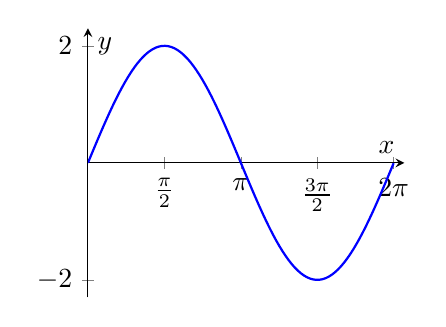
\begin{tikzpicture}
\begin{axis}[
    width=5.6cm, height=5cm,
    axis lines=middle, xlabel={$x$}, ylabel={$y$},
    xmin=0, xmax=6.5, ymin=-2.3, ymax=2.3,
    xtick={1.57,3.14,4.71,6.28},
    xticklabels={$\frac\pi2$,$\pi$,$\frac{3\pi}{2}$,$2\pi$},
    ytick={-2,2},
]
\addplot[thick,blue,domain=0:6.28,samples=100] {2*sin(deg(x))};
\end{axis}
\end{tikzpicture}
\end{column}
\end{columns}
\end{frame}

% ---------- 18 ----------
\begin{frame}[t]{拓广探索 18：由图象写解析式}
\textbf{18.} 已知函数 $y=f(x)$（$x\in\mathbf R$）是周期函数，周期为 $2$，其部分图象如图所示。
\begin{enumerate}[(1)]
  \item 写出函数 $y=f(x)$ 的解析式；
  \item 画出函数 $y=f(x+1)$ 的图象。
\end{enumerate}
\vspace{0.5em}
\begin{center}
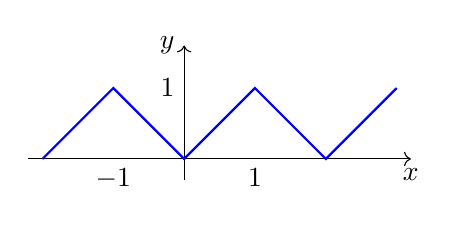
\begin{tikzpicture}[scale=0.9]
  \draw[->] (-2.2,0)--(3.2,0) node[below]{$x$};
  \draw[->] (0,-0.3)--(0,1.6) node[left]{$y$};
  \draw[thick,blue] (-2,0)--(-1,1)--(0,0)--(1,1)--(2,0)--(3,1);
  \node[below] at (-1,0) {$-1$}; \node[below] at (1,0) {$1$};
  \node[left] at (0,1) {$1$};
\end{tikzpicture}
\end{center}
\end{frame}

\begin{frame}[t]{拓广探索 18 解答}
\begin{tcolorbox}[colback=orange!10,colframe=orange,title=\textbf{解}]
(1) 在一个周期 $[0,2]$ 上，图象为三角形：$[0,1]$ 从 $(0,0)$ 升到 $(1,1)$，$[1,2]$ 从 $(1,1)$ 降到 $(2,0)$。故
\[
f(x)=
\begin{cases}
x, & x\in[0,1],\\
2-x, & x\in[1,2],
\end{cases}
\quad \text{周期为 }2.
\]
即 $f(x)=1-|x-1|$ 在 $[0,2]$ 上延拓为周期 $2$ 的三角波。
\vspace{0.3em}
(2) $y=f(x+1)$ 是把 $y=f(x)$ 的图象\alert{向左平移 $1$ 个单位}（形状不变，周期仍为 $2$）。
\end{tcolorbox}
\end{frame}

% ---------- 19 ----------
\begin{frame}[t]{拓广探索 19：对称性探究}
\textbf{19.} 正弦曲线关于原点对称，原点是它的对称中心。除原点外，正弦曲线还有其他对称中心吗？有对称轴吗？对余弦函数、正切函数，讨论上述同样的问题。
\end{frame}

\begin{frame}[t]{拓广探索 19 解答}
\begin{tcolorbox}[colback=orange!10,colframe=orange,title=\textbf{参考结论}]
\textbf{$y=\sin x$：} 对称中心为 $(k\pi,0)$；对称轴为直线 $x=\dfrac{\pi}{2}+k\pi$。
\vspace{0.2em}
\textbf{$y=\cos x$：} 对称中心为 $\left(\dfrac{\pi}{2}+k\pi,0\right)$；对称轴为直线 $x=k\pi$。
\vspace{0.2em}
\textbf{$y=\tan x$：} 对称中心为 $\left(\dfrac{k\pi}{2},0\right)$；无对称轴（它是奇函数，图象关于原点对称）。
\vspace{0.3em}
\small（理由：正弦在最值点处切线水平，为对称轴；在零点处曲线穿过，为对称中心。）
\end{tcolorbox}
\end{frame}

\begin{frame}[c]
  \begin{center}
    {\Huge\calligra Thanks!}
  \end{center}
\end{frame}

\end{document}
